\documentclass[  12pt,
titlepage,
parskip,
draft=false,
headsepline=true,
footsepline=true,
captions=tableheading]{scrartcl}
\usepackage[english]{babel}
\usepackage[utf8]{inputenc}
\usepackage[a4paper , lmargin = {2.5cm} , rmargin = {2.5cm} , tmargin = {2.5cm} , bmargin = {2.5cm}]{geometry}
\usepackage[hyphens]{url}
\usepackage[linktocpage=true]{hyperref}
\usepackage{tabularx}
\usepackage{amsmath}
\usepackage{eurosym}
\usepackage[backend=biber,style=authoryear,sortcites=false,citestyle=authoryear,url=true,natbib=true]{biblatex}
\addbibresource{Literatur.bib}%Dateiname für Quellen einfügen
\usepackage{ragged2e} %für bessere URL formatierung bei printbibliography
\usepackage{afterpage}
\usepackage{glossaries}
\setacronymstyle{long-short}
%\GlsSetQuote{+}
\makenoidxglossaries
\loadglsentries{acronyms}
%Bilder einbinden und es ermöglich auf der gleichen seite ein
%Fußnotenzitat einzufügen
\usepackage{graphicx}
\usepackage{float}
\usepackage{afterpage}
\interfootnotelinepenalty=99999 %Seitenumbruch einer Fußzeile verhindern

\newcommand{\bildcite}[5]{
	\begin{figure}[htbp]
		\centering
		\includegraphics[width=#5\textwidth]{Pictures/#1}
		\vspace{2mm}
		\caption[#2]{#2\footnotemark}
		\label{#3}
	\end{figure}
	\footnotetext{#4}
}

\usepackage{longtable}
\usepackage{moreverb} %tabulator formatierung in verbatim umgebung

%nur einzelne Kapitel einbinden:
%\includeonly{1_Introduction}
%\includeonly{2_Offshoring-Literature}
%\includeonly{3_Case-Studies}
%\includeonly{4_Conclusions}

%Change standard enumeration layers
\renewcommand{\labelenumi}{\arabic{enumi}.}
\renewcommand{\labelenumii}{\arabic{enumi}.\arabic {enumii}}
\renewcommand{\labelenumiii}{\arabic{enumi}.\arabic{enumii}.\arabic{enumiii}}

%Disable Appendix Sections showing up in ToC
\newcommand{\nocontentsline}[3]{}
\newcommand{\tocless}[2]{\bgroup\let\addcontentsline=\nocontentsline#1{#2}\egroup}

%First pages
\newcommand{\firstpages}{
	% !TEX root = Thesis.tex

\thispagestyle{empty}
\vspace{1cm}

\begin{center}
\Large{Hochschule für Telekommunikation Leipzig (FH)}
\vspace{1.5cm}
\end{center}

\begin{center}
\large{\textbf{Abschlussarbeit zur Erlangung des akademischen Grades}}
\end{center}

\begin{center}
\vspace{-2mm}
 \Large\textbf{Bachelor of Science}
\end{center}

\begin{center}
\vspace{5mm}
\textbf{im Studiengang Wirtschaftsinformatik}
\end{center}

\vspace{3cm}
\begin{tabular}{p{0.2\textwidth}p{0.7\textwidth}}
\textbf{Thema:} & 
	Exploring the offshoring approach of German Companies compared to  to the U. S. American approach

\\
&
	
\\ &
\\ &
\\

\vspace{4,5cm}\\

\textbf{Vorgelegt von:} & Veronika Lawrence \\ 
&\\
&\\
&\\
&\\
\textbf{geboren am:} & 31. Oktober 1991 \\
\textbf{in:} & Starnberg \\
\textbf{Matrikelnummer: } & {}134130\\
&\\

\textbf{eingereicht am:} & 15. Oktober 2016 \\
&\\
&\\
&\\
\textbf{Themensteller:} & T-Systems International\\
& Systems Integration\\
& SAP Technology \& Analysis\\
& \\

\textbf{Erstprüfer:} & Prof. Dr. Christian Czarnecki \\
&\\
&\\

\textbf{Zweitprüfer:} & [Titel einfügen]Thomas Vogt \\
\end{tabular}
 
	\afterpage{\blankpage}
	\newpage
	\pagenumbering{arabic}
	\setcounter{page}{3}
	\tableofcontents{}
	\addtocontents{toc}{~\hfill\textbf{Page}\par}

	\newpage
	\listoffigures
	\addcontentsline{toc}{section}{List of Figures}
	\newpage
	\listoftables
	\addcontentsline{toc}{section}{List of Tables}
}



\newcommand\blankpage{%
	\null
	\thispagestyle{empty}%
	\newpage}

\begin{document}
\pagenumbering{gobble}
\firstpages
\newpage
\addcontentsline{toc}{section}{List of Acronyms}
\printnoidxglossary[type=\acronymtype,title={List of Acronyms},sort=use, nogroupskip=true, nopostdot=true]

% !TEX root = Thesis.tex
\section{Introduction}
In the past two decades, globalization has changed the structure of markets worldwide. Whole countries specialize and build their strengths. For example, India has developed into the global IT development and support powerhouse to the extent that many companies from other countries have relocated these tasks to either their own Indian subsidiary or an external Indian company.

Germany is traditionally a country with very strong exports. Therefore, the German economy has profited from globalization. But high labor cost in Germany is a problem for many companies. They tried to solve this in a similar way many American companies have successfully lowered their labor cost, through shifting tasks to a different country with lower labor cost. This is called offshoring.

One of the main drivers for offshoring is cost, but other considerations such as the development of new markets, strategic concerns or fiscal incentives play also a big role in inspiring companies to offshore. In figure \ref{fig:GERMotives}, the results of a survey conducted by German \textit{Statistisches Bundesamt} regarding the motives of German service companies for offshoring are illustrated. Labor and other cost are two of the top three arguments for offshoring, considerations of strategic or fiscal nature are less important. The least relevant motivators are less business regulation in the offshoring destination and following customers or competitors offshore.

\vspace{5mm}
\bildcite{GER_Motives}{Motives to offshoring of German service companies}{fig:GERMotives}{Data source: \cite[pp. 26f]{StatistischesBundesamt.2008}}{0.7}


%ACHTUNG Hier fehlt noch was für den roten Faden: job loss <-> 20% der high knowledge service jobs mehr nach offshoring als vorher, wenn qualifiziert

By the German as well as the U.S. general public, offshoring plans are often dismissed as a selfish move of profit-hungry corporations. Employees fear for their job security and politicians criticize the job loss that offshoring entails. Contrary to these objections, research has shown for the U.S. that there is no evidence indicating that jobs are shifted abroad in a quantity that is discernible on nation-wide statistic trends (\cite[p. 7]{Jackson.2013}). Similarly, in 2005 only 7.2 \% of total German job losses were connected to offshoring (\cite[p. 30]{Gorg.2011}).

The survey mentioned above even found a positive employment effect for qualified jobs in the service industry. For the explored time frame, 20\% more jobs have been created than those that have been offshored previously. For less qualified jobs, 75.9 \% of shifted jobs have been compensated through the creation of new jobs. (\cite[pp. 21f]{StatistischesBundesamt.2008})

This shows that the fear of the general public is not warranted, even though offshoring may certainly have a profound effect on individual persons. But on the larger scale, offshoring improves productivity of countries (\cite[pp. 90f]{Jahns.2007}).

Additionally to resistance to offshoring from German society, especially from unions and worker's councils, offshoring ventures of German companies have often faced  problems and project failures. In contrast, American companies have been more successful.

There is a plethora of existing research of offshoring, separate for German and American companies, but rarely are both directly compared (one example is \cite{Hutzschenreuter.2007}). The reasons for existing differences are even less explored.
\vspace{3mm}

The goal of this thesis is answering the question:

\begin{quote}
	\centering \textbf{What are the differences regarding IT offshoring between German and U.S. companies, and how can they be explained?}
\end{quote}
\vspace{3mm}

In order to achieve this goal, the thesis will include an analysis on available literature on the topic. Research will be conducted in the libraries of \textit{Hochschule für Technik, Wirtschaft und Kultur Leipzig} and \textit{Ludwig-Maximilians-Universität München}. Additionally, online resources like \textit{Google Scholar} or \textit{SpringerLink} will be utilized to find relevant literature. 

The findings of this analysis can be found in section \ref{sec:Theory}. In this section, relevant terms will be defined, before exploring factors for offshoring in general and specifically for the U.S. and Germany. The last subsection contains a direct comparison of both countries.

The results of theoretical research will be extended through the conduction of expert interviews with interview partners, that have extensive experience with offshoring in the IT industry from different points of view. This empirical research will complement the theoretical findings with real-world knowledge and experience. Further reasons for the different offshoring results of U.S and German companies will be uncovered, adding new, unique knowledge to the existing body of research.

In section \ref{sec:Empiry}, the interview process is described in order to enable further research achieve comparability to the work that is described in this thesis. The following four subsections describe the results of the expert interviews, each subdivided into a section about the expert's background, a section describing the results of the interview and a final section with conclusions that can be drawn from the interview. The final subsection summarizes the findings from all interviews.

The scope of the empirical part of the thesis is limited to the IT industry for reasons of clarity and availability of experts for interviews. In the theoretical section \ref{sec:Theory}, data is analyzed for all industries.

In this thesis, production is not considered a part of offshoring. As detailed in section \ref{sec:DefTerms}, offshoring is a shift of tasks and does not involve shipment of physical goods. Furthermore, offshoring with the exclusive goal of tax evasion is not a subject of this thesis.



% !TEX root = Thesis.tex
\section{Offshoring in literature}
Offshoring has been widely studied in the past decades. There are two major branches of research: the first describes reality through statistics or case studies (e.g. \cite{Rottman.2008}, \cite{Pedersen.2013} )

\subsection{Definition and Terms}
In existing literature, there is no single definition of the term offshoring nor a precise delimitation to the term outsourcing. Both apply to organizational decisions in companies. 

According to \cite[pp. 1f]{Specht.2007}, outsourcing is buying services from other companies. Offshoring is defined as a special form of outsourcing, in which the service is bought from a foreign company. \cite[p. 2]{Alebrand.2013} defines outsourcing and offshoring as mutually exclusive: outsourcing is the provision of services by external companies, offshoring is the internal execution of tasks in a foreign country.

These contrasting definitions may serve as an example for the lack of distinct terms in this field of research. Nevertheless all the definitions agree that outsourcing pertains to external service provision and offshoring refers to service provision in a foreign country. This synopsis as well as the planned Bachelor's thesis will use the following definition of the term offshoring by \cite[p. 321]{Andersson.2016}:

%\begin{quote}
%	``Offshoring [is the] disintegration of the firms’ production processes across national borders[...]''
%\end{quote} 

Therefore, the terms offshoring and outsourcing do not have a direct relation; both terms are independent and describe different possibilities of entrepreneurial organization. In figure \ref{fig:DefTerms}, the delimitation between outsourcing and offshoring is clearly shown.

\begin{figure}[htb]
	\centering
	\includegraphics[width=0.7\textwidth]{Pictures/Terms_definition}
	\caption{Definition of terms, based on \cite[pp. 552f]{Antras.2004}}
	\label{fig:DefTerms}
\end{figure}



\subsection{History of Offshoring}
%Enabling Technologies
%

\subsection{Offshoring in the USA}

\subsubsection{Prevalence}

\subsubsection{Offshoring functions}

\subsection{Offshoring in Germany}

\subsubsection{Prevalence}

\subsubsection{Offshored functions}

\subsection{Significant differences between Germany and the USA}

\subsubsection{Difference 1}

\subsubsection{Difference 2}


% !TEX root = Thesis.tex

\section{Case Studies}

In order to expand on existing knowledge, a series of expert interviews has been conducted for this thesis. In the following section, the process of conducting the interviews is described. Next, there is an in-depth summary of each interview, concluded by an abstract to highlight the most important points for this thesis. The last section contains a comparison and evaluation of all interviews.

\subsection{Interview Technique}
%TODO evtl kürzer fassen
In order to complement theoretical findings from literature research, expert interviews have been conducted. A structure for the interviews has been defined (see appendix). In this way, statements from different experts can be compared and evaluated, which allows for a comprehensive review. Even though interviewees may share their native language (German) with the interviewer, interviews have always been conducted in English. Thus, any inaccuracies that may occur during translating the statements were prevented and comparability of interviews has been improved.

The interviews were held remotely, either via an Internet VoIP-Service such as Skype, or via using WebEx, the standard communication platform used at T-Systems when interviewing employees of this company. Considering the often tight schedules of experts in their fields, the duration of interviews was planned to be 45 minutes.

To further document the interviews and the steps leading up to them as well as the steps of refinement that follow, a process (see figure \ref{fig:Intprocess}) has been defined and adhered to. 

\vspace{3mm}
\begin{figure}[htb]
	\centering
	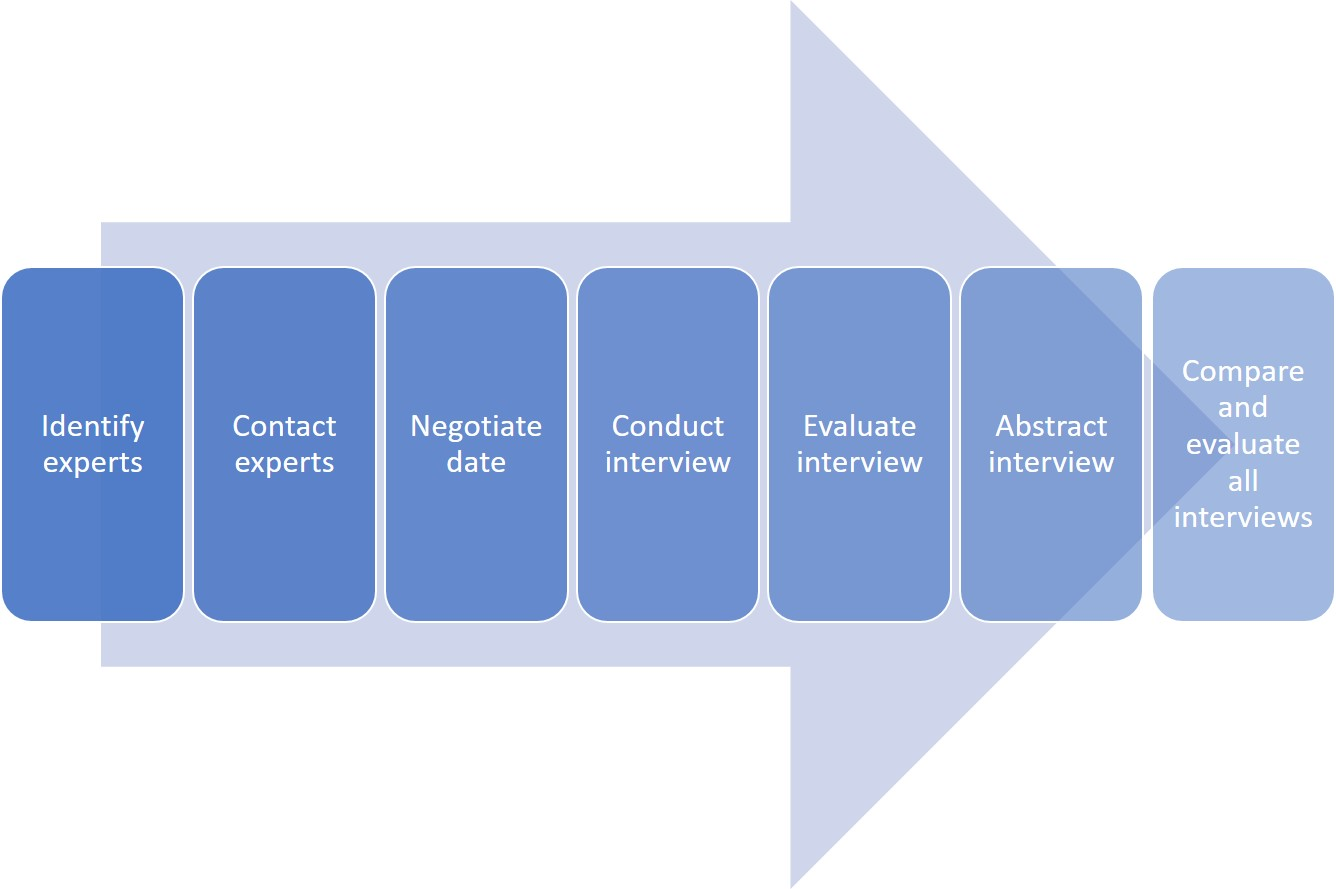
\includegraphics[width=0.85\textwidth]{Pictures/Interview_process}
	\caption{Interview process}
	\label{fig:Intprocess}
\end{figure}

\newpage

\paragraph{Identify experts} The experts are identified by conducting a network-based search. Initial contacts are asked to identify persons they consider an expert on the topic, who are in turn asked to provide further contacts.
\paragraph{Contact experts} Initial contact to the expert is established via an email sent by the expert's contact. Included is a standard email explaining the topic, duration and process of the interview and providing the researchers' contact details.
\paragraph{Negotiate date} Once the expert has agreed to participate in the interview, the researcher contacts them directly in order to set up date, time and method of communication for the interview. Note that all interviews are conducted using at least voice-based communication. Video can be added to further facilitate the communication between the expert and the researcher.
\paragraph{Conduct interview} The interviews are conducted in five phases with defined leading questions\footnote{The structure of the interview can be found in the appendix, page \pageref{app:InterviewStructure}.}. This means, the leading questions will be asked, but the researcher will also ask further questions as appropriate to the course of the interview. These phases are:
\begin{itemize}
	\item Introduction
	\item Offshoring Experiences in the USA
	\item Offshoring Experiences in Germany
	\item Comparison of Experiences in Germany and the USA
	\item Finalization
\end{itemize}
During the interview, audio has been recorded. The audio files form the primary source of knowledge gained from the experts.


\paragraph{Evaluate interview} The recordings are evaluated and any important passages are noted. These evaluations are added to the appendix.

\paragraph{Abstract interview} For each interview, an abstract is developed. The abstracts are included in the thesis.

\paragraph{Compare and evaluate all interviews} Finally, an overview and comparison of all interviews is generated to derive common statements and areas of disagreement.

\newpage
\subsection{A German Project Manager on Offshoring with Different Service Providers}

This interview was conducted on 1. July 2016 08:00 h CEST with Michael Scheitza, a senior project manager at T-Systems International. The standard communication tool of T-Systems, Cisco WebEx, was used for the interview. The recording of the interview can be found on the enclosed CD (file name: 20160701\_Michael\_Scheitza.mp3). A written summary of the interview is found in appendix, page \pageref{int:Scheitza}.

\subsubsection{Background}
Michael Scheitza has worked for eight years as a project manager in an international environment. He has experience in offshoring projects with Russia, Poland, Romania, India, Malaysia, Mexico, and Brazil. He does not have any experience with offshoring from a U.S. perspective, so he did not feel comfortable answering any questions regarding this topic. 
\subsubsection{Results of Interview}
At T-Systems, application management contracts are often delivered offshore. Most customers leave the choice of delivery location to T-Systems, provided there is no legal obligation to deliver locally. The delivery model for each contract is chosen by the necessary skills, the language that is requested by the customer, and required service levels. When deciding on a delivery location, scalability is very important. It is essential that there are enough people with the required knowledge.

Generally speaking, there are two different possible working relationships between customer, German on-site team and offshore team. %Bilder hier einfügen

\vspace{3mm}
\begin{figure}[htbp]
	\centering
	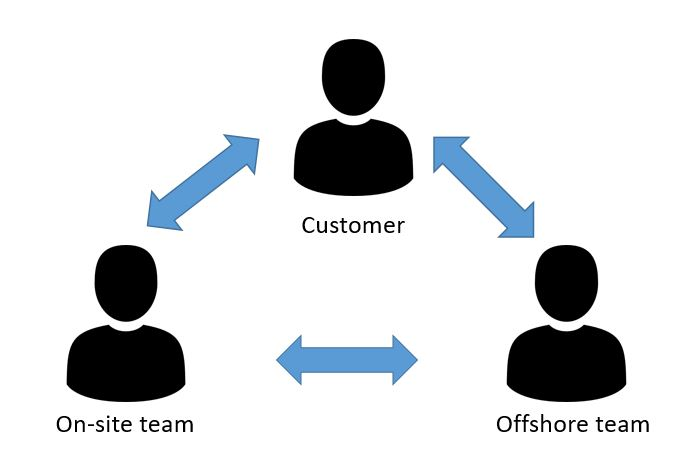
\includegraphics[width=0.5\textwidth]{Pictures/1on1_relationship}
	\caption{Direct, personal relationships between customer, on-site team and offshore team}
	\label{fig:1on1}
\end{figure}

The first possible working relationship works best in teams smaller than 50 persons offshore. In the transition phase, offshore team members travel to Germany in order to directly interact with and learn from the customer. In figure \ref{fig:1on1}, the set up in this case is depicted.

The interviewee gave an example of an application management contract that was delivered from Brazil. There was the requirement that all 20 team members speak enough German to directly speak to the customer. In transition phase, personal relationships were established between the Brazilian team, the customer and German project management of T-Systems. This facilitated collaboration later in the project, because the persons involved knew each other in person, not only via telephone and email.

The motivation for the offshore team in this case stems from the identification as part of a global delivery team. If the on-site and offshore teams share the same tasks, the delivery model is called \textit{Verl\"angerte Werkbank}. The team size in this case is usually less than 30 people and the project manager distributes tasks directly to offshore team members. 

The drawback in this approach is that it tends to increase volatility in the team. Michael Scheitza shared an experience he made with an Indian team: Each time there were quality issues, T-Systems had spent money on bringing team members on-site or German project management had traveled to India to improve communication. Few months later, he noticed that especially those team members who had been to Germany left the project and changed jobs in order to further their careers. This way, the investment in communication was unsuccessful.

\vspace{3mm}
\begin{figure}[htbp]
	\centering
	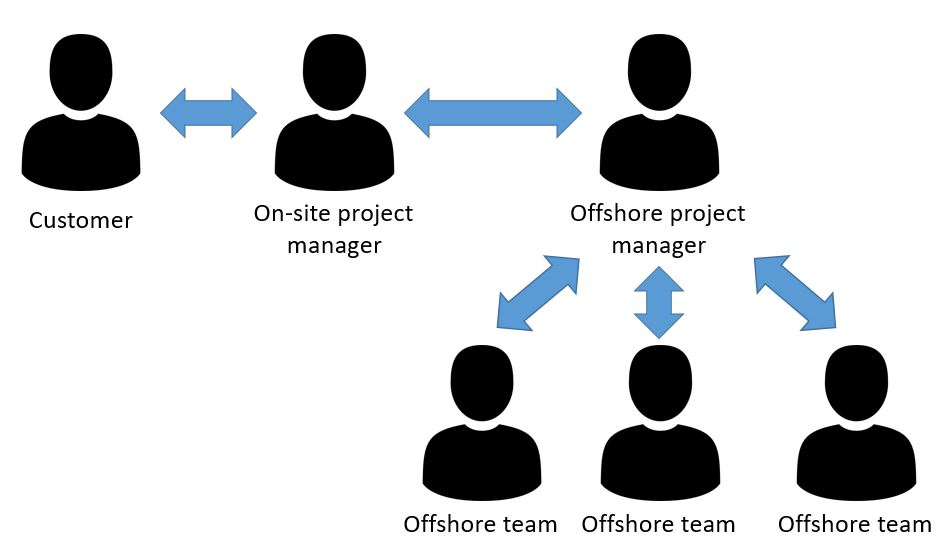
\includegraphics[width=0.7\textwidth]{Pictures/Hierarchy}
	\caption{Hierarchical communication between customer and offshore team}
	\label{fig:hierarchy}
\end{figure}

The second possibility is used in larger teams with more than 50 people. Teams that size are large enough to be organized in hierarchical layers with a local team lead or project management. This approach does not involve deep relationships and personal communication. Instead, the working relationship is managed via \glspl{sla} and \glspl{kpi}, where quality and quantity of deliverables are defined. The communication structure in this case is depicted in figure \ref{fig:hierarchy}. In transition phases of projects, only the offshore project managers or team leads travel to Germany and distribute the knowledge they gained in working with the customer to their teams offshore.

In this case, the offshore team does not identify as a part of a global delivery team, because the personal relationships that are needed for this approach are not in place. Alternately, the team members can identify with the project itself and are motivated by the local project manager. Ideally, the team is driven by the desire to be successful in fulfilling the contract.

Neither approach, said Michael Scheitza, is clearly superior to the other. Each has its drawbacks and advantages, and both are applicable in certain situations.

\subsubsection{Conclusions}

In the interview, Michael Scheitza differentiated and specified two distinct approaches to offshoring that are used in Germany. In table \ref{tab:ScheitzaApproaches}, they are directly compared to each other. 
\vspace{3mm}
\begin{table}[htb]
	\centering
	\begin{tabular}{l|p{5.8cm}|p{5.8cm}}
		& \textbf{Personal Relationships} & \textbf{Numbers-based Approach}\\\hline
		
		\rule{0pt}{3ex}Team size &$<$ 50 people &$>$ 50 people\\ \hline
		\rule{0pt}{3ex}Transition phase&All offshore team members travel on-site and form personal relationships with T-Systems team members and customers &Offshore project managers travel on-site and share their knowledge with the team\\ \hline
		\rule{0pt}{3ex}Communication &Direct communication between customer, on-site team and offshore team & Hierarchical communication from customer to on-site team to offshore project management to offshore team \\ \hline
		\rule{0pt}{3ex}Motivation &Identification as part of a global delivery team &Motivation by local project management and identification with the contract \\ \hline
	\end{tabular}
		\vspace{3mm}
		%Immer caption vor label!!!
		\caption{Comparison of German offshoring approaches according to M. Scheitza}
		\label{tab:ScheitzaApproaches}
\end{table}

Even though the interviewee could not contribute any experience with offshoring from an American point of view, there have been very interesting points. Firstly, the other interviews focused mainly on offshoring with an Indian service provider. This interview offered insights in offshoring projects with a multitude of different destinations. Secondly, there were criteria for choosing a delivery model outlined. Last, the two different collaboration models were described very thoroughly, offering a concise view on the offshoring projects the interviewee experienced.


\subsection{An Indian Offshoring Pioneer Comparing German and U.S. Clients}
A. S. Viswanathan agreed to be interviewed on 7. July 2016 at 17:00 h CEST / 20:30 h IST. For this, Skype was used as a communication tool. On the enclosed CD, the recording of the interview has the file name 20160707\_A\_S\_Viswanathan.mp3. The summary of the conversation can be found in appendix page \pageref{int:Viswanathan}.
\subsubsection{Background}
The interviewee is electrical engineer with a specialization in industrial engineering. In 1978, he started his career with English Electric, which was a part of General Electric Group. There, he worked for two years before joining Siemens. With Siemens, he held various positions ranging from the shop floor to CIO of the IT subsidiary of Siemens in India. Later, he moved on to the board of Siemens Information Systems, a software company that took global mandate within the Siemens Group. His responsibilities included Business Solutions for offshoring SAP, which his team was pioneering in India, as well as IT services.

In 2007, Siemens merged all local IT companies into a new company called IT Services and Solutions. Viswanathan was on the executive management of this company, heading Global Portfolio of Mobility.

After taking a break in 2011, he founded his own management consultation company in 2012. He specializes in offshoring consulting, primarily with customers from Germany, China and India.

\subsubsection{Results of Interview}
\paragraph{Offshoring in the U.S.}When first conceptualizing the offer of offshoring services, the first customers were from the United States. They were very quick in understanding the advantages and seizing the opportunity, not only shifting single tasks, but entire operations to India. Before offshoring, U.S. companies took the time to evaluate different service providers. Once the decision was made, there was no plan B, so there was a necessity to make offshoring work.

This has a profound effect on working relationship. In Viswanathans experience, contributing to positive working relationships was English being a common language. Management meetings and schedules were easily set up. \Glspl{sla} were more critical, as after the initial cycles of new contracts, there would be a new wave of requirements, imposing stricter quality standards. In this phase, facts and figures dominate the working relationship.

The American approach to offshoring is characterized by legalistic and contractual concerns. When researching service providers, U.S. companies have consultants performing background searches of companies providing operations in India. Three to four companies are shortlisted and visited by the American team for presentations. Thereafter, contract negotiations start. A lot of emphasis is placed on contracting and commercial \glspl{sla}. The processes are not deemed as important, since the companies believed in the ability of the service provider to deliver.

Contributing to the success of American offshoring projects is the high offshorability of an American job. The work is conceptualized as a specific set of tasks where a specific set of skills is needed. Therefore, the skills of workforce can easily be managed. This goes back to U.S. companies already have experience with shifting jobs within the U.S. and people are already working in different places and time zones within the country. Also, jobs are very transaction-based in the U.S.. The education system facilitates that each employee does not need to have an end-to-end knowledge of the entire process. This is connected to the higher fluctuation of employees in American companies and is a huge advantage when it comes to offshoring -- it needs only minimal training to enable a new person to do the job.

\paragraph{Offshoring in Germany}Compared to American jobs, in German companies the job design is much more intrinsic and process-oriented. An example of a buyer is given: in Germany, the buyer has a specific background in the field, maybe an apprenticeship or some other kind of special training, whereas the buyer in the U.S. is not expected to have deep insights in the field when starting the job. The German buyer has knowledge in costing, the market, and product design, whereas the American buyer consults a technical specialist for those details. This system-oriented thinking is an advantage for the German society, but an obstacle for offshoring.

This kind of job design is mirrored in the SAP systems of companies. When it comes to customizing the system, a German system differs greatly from an American system, because the role of an individual is more holistic in Germany. This presents a problem when shifting tasks offshore, as one person in Germany can't simply be replaced by one person in India as it is the case with American jobs. The person in India simply lacks the specific background and experience with the German company.

Furthermore, offshoring is a very alien concept for German companies, especially \gls{sme}. Those grow very organically from small family businesses, so the owners have in-built control of all processes from the beginning. When it comes to outsourcing within Germany, the service provider does not have full control of the entire process, but only provides some parts. Additionally, German service providers often have a very good knowledge of their customers, and are almost an extension of their customers' organization. 

When it comes to offshoring, both of these points present problems. When relocating tasks, the customer inevitably needs to give up control over processes. Similarly, when replacing domestic outsourcing with an offshore provider, the same standard can not be applied to a foreign company that is used to evaluate a German company that has years of experience collaborating with the customer. Additionally, Germans tend to display a high degree of detailing, so the standards for the service providers are often very high. This has, in Viswanathan's experience, been one of th biggest barriers for German companies approaching offshoring, and it is important to achieve a change in mindset for this. Also, in general Germans are more used to exporting than to importing. The notion to import services from a different country is somewhat foreign, as it implies that the service provider could do the job better than the German company itself.

It is very typical of German companies to prefer \gls{fdi} over foreign outsourcing. Frequently, an implicit objective is recreating the own organization in India. The reason for this is the inability of German companies to change the structure of jobs in a way that makes them easily offshorable.

Language is a further important point that must be discussed when talking about offshoring in Germany. German companies are becoming more international, but many still prefer to have their systems built and maintained completely in German. This is becoming less of a problem as many Indians are learning German, but it still is a handicap.

Additionally, the transition phase must be carefully managed when implementing offshoring, especially with respect to the loss of jobs or the decrease of job security in the German company. Work councils and unions make this process slow and difficult. This needs to be accepted and accounted for in the planning both on the German and Indian side. A comparable American company would be much quicker in implementing offshoring, which is a tremendous disadvantage for German companies. In the worst case, Viswanathan recounts, shortly before completing the transition, unions had objected to an offshoring project so all measures had to be reversed. This was a very difficult scenario for both the service provider and the customer, as the setup in India was already completed.

A German company that wants to offshore successfully first needs to define entire functions that can be offshored, rather than offshoring just some minor roles. Second, if the company is looking to offshore not only easily offshorable IT services\footnote{Hardware, infrastructure support and similar tasks}, but business processes, they must be designed in a way that the transactions are separated from the decision-making. Then, the transaction part of the job can be offshored without many problems. However, as long as jobs are looked at in an integral way, it is an obstacle to offshoring. The very deep level of job ``slice and dice'' that is common in American jobs is not needed, but that one level of division could help German companies to more success in offshoring.

Application management is identified as one function that is easily offshorable. In general, the tasks could be dealt with replacing one German resource with three Indian resources. This, of course, results in a much smaller cost arbitrage but still yields an economic advantage as multitasking can be applied in the Indian site. The distribution of work is managed by Indian managers who have enough knowledge of the entire process in this scenario. Obviously, this is a lot more management effort than offshoring with an American companies would entail.

\subsubsection{Conclusions}
In this interview, Viswanathan described the very different experiences he had with German and American clients. Many of his points are supported by literature research as laid out in section \ref{sec:Theory}. To recap his statements, in table \ref{tab:ViswanathanComparison} the German and American approach to offshoring according to A. S. Viswanathan are analyzed.

\vspace{3mm}
\begin{table}[htb]
	\centering
	\begin{tabular}{l|p{5.55cm}|p{5.55cm}}
		& \textbf{U.S.} & \textbf{Germany}\\\hline
		\rule{0pt}{3ex}Job design& Transaction-based, no need of end-to-end process knowledge, specific set of tasks with deep level of  &Holistic, process-oriented task which require extensive domain knowledge\\ \hline
		\rule{0pt}{3ex}Employee education&Minimal training &Specialized vocational training, apprenticeship or academic background and years of experience in the company \\ \hline
		\rule{0pt}{3ex}Offshoring approach&Contractual and legalistic focus when setting up offshoring; Emphasis on \glspl{sla} &\gls{fdi} is preferred in order to recreate the own organization in the offshoring destination \\ \hline
		\rule{0pt}{3ex}Expectations&Quality is adjusted in multiple waves of requirements &Very high quality standards from the start\\ \hline
		\rule{0pt}{3ex}Shifting ratio& One American resource to one Indian resource & One German resource to three Indian resource\\ \hline
		\rule{0pt}{3ex}Language&Facilitates communication and collaboration &Rare skill offshore, hard to learn \\ \hline
	\end{tabular}
	\vspace{3mm}
	%Immer caption vor label!!!
	\caption{A. S. Viswanathan's comparison of American and German approaches to offshoring}
	\label{tab:ViswanathanComparison}
\end{table}

As shown in the table, German companies in comparison to American have quite a few obstacles to overcome in order to successfully offshore. Some of the characteristics that are unique to German companies and have often proved to be an competitive advantage in global markets are at the same time a disadvantage for offshoring. The most important point is here the difference in job design. 

A. S. Viswanathan provided the vast knowledge and experience with offshoring he has gained over the course of his career in this interview. In a pointed way, he determined the differences of American and German companies when it comes to offshoring. Having worked with both American and German clients, he is in a unique position for making this comparison.

\subsection{Ingo K\"ummritz}
The interview with Ingo K\"ummritz took place on 03. August 2016 at 10:00 h CEST. As a communication tool, Skype was used. The file name of the audio recording on the enclosed CD is 20160804\_Ingo\_K\"ummritz. The written summary is in appendix, page \pageref{int:Ingo}.

\subsubsection{Background}
Ingo is German, but went to High School and College in the U.S., which has helped him broaden his horizon when it comes to international delivery. In 2003 he was working at IBM and the country manager approached him, offering him to take responsibility for global delivery. In this time, he was in the role of a principal, which is a topic expert within the IBM organization. Later, after 10 years of working at IBM, he switched jobs and started with Siemens, moving to a customer-facing role. Several years later, he had a short contract at an Indian company and ended up at NTT Data in Germany afterwards. At present, he holds a subject matter expert role again.

All in all, Ingo has been working in the area of global delivery for 13 years, mostly with India. In this time, he was responsible for large projects and \gls{ams} deals in delivery, sales, and customer-facing positions. This has helped him to understand all partners involved better. In offshoring projects, he has been both in integrated delivery teams and in customer teams that traveled to India to set up offshoring there. His experience pertains to \gls{fdi} only. Whenever he has worked with an Indian team, they were his colleagues at IBM or Siemens.

Even though he does not have first-hand experience with offshoring from an U.S. perspective, he spent quite some time there and had many American colleagues, considering IBM is an American company. In a way, the work they did at the German subsidiary of IBM could be considered offshoring by the American headquarter.

\subsubsection{Results of Interview}
When talking about global delivery, there is no dedicated location for delivery, but rather a delivering company. This company needs to find the right delivery model with regard to resources and locations. The right location is not necessarily India, but this country is the global powerhouse in the \gls{ict} industry. About 90\% of the projects and services that included offshoring in Ingo's experience involved the Indian subsidiary. The time zones are very convenient for offshoring, as well, because Central European business hours can be covered from India without needing to use late shifts.

The critical point, regardless of the type of work that is being offshored, is communication and cooperation. It is critical to learn how the counterpart on the service provider side is thinking and reacting to communication. Rather than processes, methods and tools, interaction is the critical factor in offshoring. Still, the right processes, methods and tools are the basis for successful work in Germany or in an international context.

\paragraph{Offshoring in the U.S.}
There are two main drivers to offshoring in the U.S., to Ingo's knowledge. One of those drivers is the cost arbitrage between employing Indian and American administrators or IT engineers. In U.S. companies, the willingness to take risks in order to take advantage of this is generally quite high when compared to German companies. The second driver is for companies not involved in the IT industry, there is often a high volatility in the business behavior. There need to be large teams set up on short notice and the hiring process takes just too long in the U.S., especially when the needed skills are uncommon. Instead, the company shifts the tasks offshore. For example, DHL used to employ 4000 Indians from Infosys, an Indian-based company, in the U.S.. Then, after Deutsche Post bought the company, service providers were consolidated and did not include Infosys any more. This shows the different approach to offshoring of German and American companies. Business plans of new ventures in the U.S. almost always include out-tasking certain areas.

Supporting this willingness of American companies to offshore is the tendency of having a much higher tolerance for software code that is not 100\% perfect, but performs fast, than engineering-oriented civilizations such as Germany, Switzerland, or Nordic countries. This is a sign of a dedication to get new products to the market quickly. American companies are not as concerned about failures as German companies. If a new product fails at an American company, they analyze the mistakes that have been made and start over, whereas German companies try to avoid failures.

But there is not only a demand of American companies seeking to offshore, but also a supply of Indians that like to be working for American companies. Indians have adopted the American way of building their career and CVs based on the reputation of their employers, so they love to join Indian subsidiaries of companies like Dell, HP, IBM, Accenture, or one of the top-tier Indian service providers like Infosys. Also, there is no language barrier between the U.S. and India,  as English is an official language in India. Both of those factors contribute to the low barriers American companies face when setting up offshoring.

When it comes to working relationships between American companies and their service providers, there are two main possibilities. The first is a numbers-based approach, where the tasks are handed over and the service provider is managed like a subcontractor, so there is not much of an involvement on a technical or personal level. The other is the approach of building an integrated team. In this three-tier delivery model, on-site staff, people from India on-site and people offshore are working together with defined roles and rotations. Working in this way builds more of a partnership between the customer and the service provider. Both of these approaches work well in the appropriate circumstances. From the customer's perspective, there is also the additional possibility of hiring a global delivery company and collaborating only on a strategic level. The service provider then decides on delivery model and locations.

American companies are better at utilizing dedicated offshore centers. Those are dedicated teams offshore that are reserved for a certain customer. When this customer is an American company, they will get very creative in finding extra work for the offshore team to keep them occupied. In this way, tasks that keep getting postponed because there are more urgent issues at hand will be completed, even if those tasks are not in the initial scope of the offshoring project. American companies approach offshoring centers with a certain level of trust and are willing to pay for the reserved manpower in case something urgent needs to be done. 

An example for this is when Ingo was working for IBM, he needed some Indian SAP experts for an upcoming project. He approached the head of the SAP resources in India, he was told there was no one available, because of the 250 people with the required skills, 50 were in existing projects, and 200 were reserved by the American part of IBM. So Ingo could not get anyone for his project, and he thought that it was incredible to have such manpower on the bench, waiting for new projects. Nobody from the German part of IBM was willing to operate likewise, ramping up an Indian team months in advance in order to be able to engage once a new project started.

\paragraph{Offshoring in Germany}
When offshoring started to take off in Germany, there was a myth about offshoring in India that Indians are great and able to deliver any task, based on only the requirement documentation. Of course, there are many highly-skilled professionals in India, and of course, they will deliver when given a task, but that does not imply that all projects where something is delivered are successful. German companies, in the beginning, approached Indians as they would a German factory worker, handing over documentation and checking for results a few weeks or months later. This does not work with India.

So German companies needed to learn how to deal, on a partnership level, with Indians. The first attempts were talking to the service provider once in a while during the projects. When the Indian colleagues were asked if they understood the documentation, they assured that they did, but the projects still failed.

The next wave of learning included trying to understand the cultural background of the Indian colleagues better. When asked to perform a task, they would confirm they could do it because they did not want to fail their customer, regardless if they could actually deliver or not. A German would protest if they could not complete a task because of missing skills or a too small time frame, so German companies assumed Indians would do the same.

Once German teams learned how to hand over tasks to India, check for results and employ trust, they could build an integrated team with the Indian colleagues. With this approach, projects succeeded, and the integrated teams continued to succeed for a long time, because the mutual level of trust and understanding was a great motivation for all participants.

From the Indian side, service providers have made the effort to understand their German customers better, as well. They founded small centers in Germany and hired local people who could make a bridge between India and Germany, in order to be more successful in Germany.

Of course, language is an important factor when talking about offshoring in Germany. Volkswagen, for example, insists on their IT systems being built and managed completely in German. Additionally, they place a lot of emphasis on project teams being directly on-site their headquarters in Wolfsburg. So for a multi-million euro project there are 150 IT engineers needed, of which 100 need to be fluent in German. This creates huge problems with staffing. BMW, on the other hand, is more international and even requires Chinese in some German positions. The Chinese market has become very important for them.

Many Germans, especially the demographic over 45 years, are not very confident in their English skills. They know the language, but they fear making mistakes when using it, particularly in spoken communication. This creates the feeling that they are exploitable and their communication partner will use this weakness to win negotiations. The only way to improve this insecurity is exposing people to situations where they can use the foreign language without high stakes or pressure.

When trying to set up \gls{fdi} in India, many German companies face the problem that they do not have a brand in India and are not known by the general public. This is an obstacle in attracting enough skilled resources for new offshore centers.

German companies, compared to American companies, are hesitant with using dedicated delivery centers. They do not want to pay for 100 people when the tasks in scope only require 20. This hesitation might stem from a lack of trust on the German side. Also, Germany generally has a risk-avoiding culture which may be aggravating this. Risk-avoiding in this context does not mean that no risks are taken, but German companies have a tendency to perform several rounds of risk-assessment and the need to collect as much information as possible in order to correctly evaluate risks before they are accepted.

Meeting culture in Germany is based on a round-table mentality: everybody gets to contribute their opinion on an upcoming decision. This often prolongs the decision-making process. On the other hand, the quality of decisions in German companies is often very good, as many people have contributed their knowledge.

Germany is a society where an engineer approach to problems is deeply ingrained in the culture. There is a desire to learn why something does not work. As the first bank institutions ran into problems when they started offshoring, they found that their local experts did not get as much relief as anticipated, because offshoring came with additional management overhead. When they switched to integrated teams, they could reduce the communication gap and increase the success rate of projects. Many German companies have gone through the same learning process since, and most have arrived at the integrated team approach as the most successful delivery model.

German companies have needed a long time and lots of experience to learn how to implement offshoring, to use checks and balances, to have a communication plan and how to deal with the Indian colleagues. Once these are in place, offshoring can work very well for a long time in German companies. Ingo's key statement is: ``If you are capable of combining German engineering and Indian enthusiasm, then you have a successful team.''

\subsubsection{Conclusions}



\subsection{Subir Purkayastha}
\subsubsection{Background}
\subsubsection{Results of Interview}
\subsubsection{Conclusions}


\subsection{Summary and Evaluation}


% !TEX root = Thesis.tex

\section{Conclusions and Limitations}


In this final section, the findings from theoretical and empirical research will be summarized and put into context. The research question from section \ref{sec:Intro} will be answered. In the following paragraphs, some common objections to offshoring will be explored, before reviewing the method used in the thesis.

\paragraph{Summary of findings}
In figure \ref{fig:ThesisResults}, the main points from literature research, empirical work and their connection are shown. On the bottom layer, the reasons for differences in offshoring that result from literature research are listed. Hereby, neighboring triangles are connected to each other. Those with a horizontal base are a prerequisite for the inverted triangles. In an analogous manner, the second layer shows the results that have been uncovered in the expert interviews. The arrangement of the triangles shows, again, relations between neighboring elements.

\begin{figure}[htb]
	\centering
	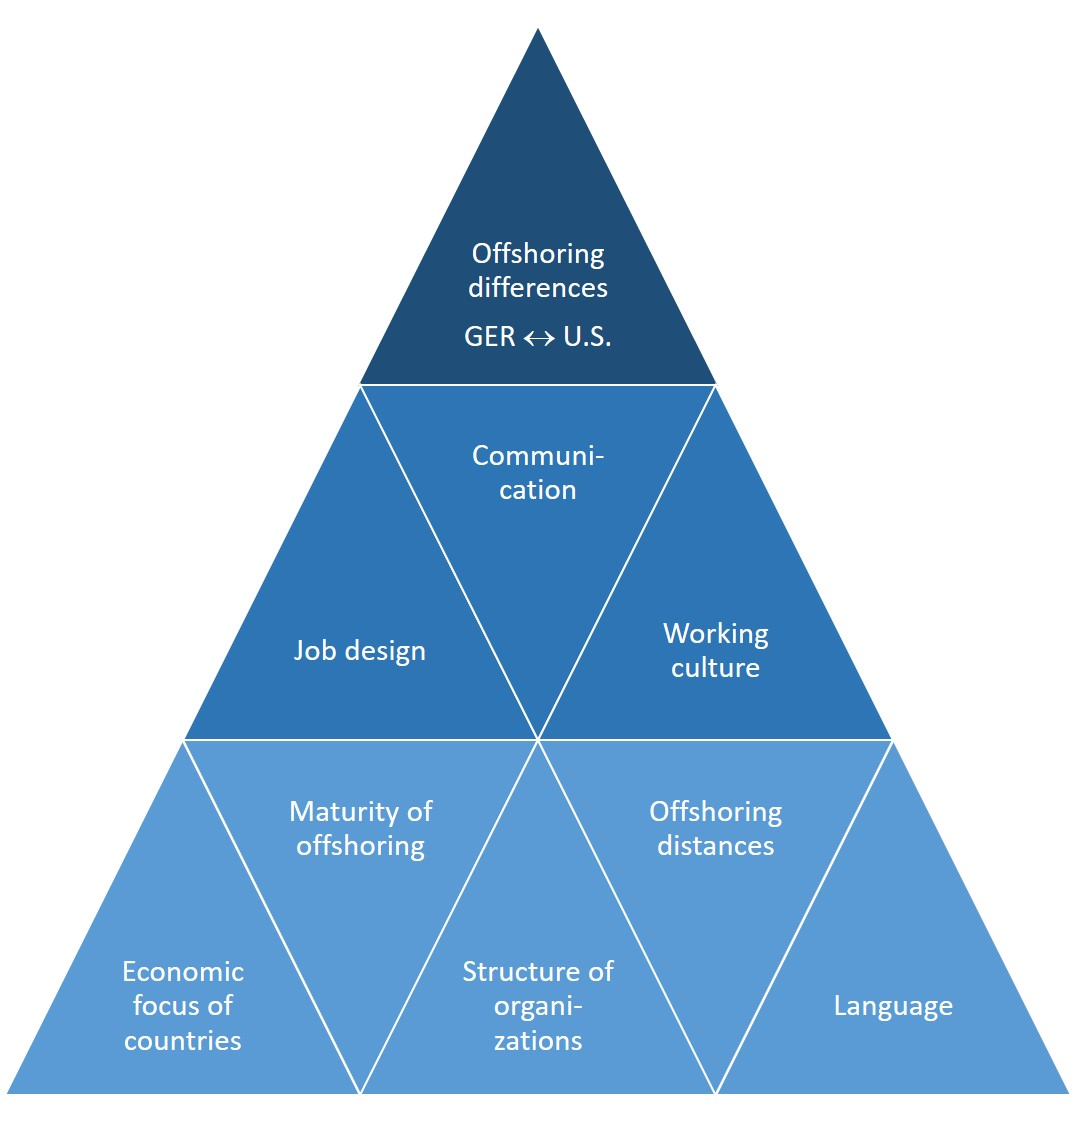
\includegraphics[width=0.8\textwidth]{Pictures/Results}
	\caption{Findings from literature research and expert interviews}
	\label{fig:ThesisResults}
\end{figure}

For example, the high maturity of offshoring in the U.S. is rooted in the prevalence of very large companies (structure of organizations) and the import focus of U.S. economy as shown in section \ref{sec:OffshoringUS}. Job design from the layer above is another important facilitator to the maturity of offshoring and a prerequisite to the unique style of communication U.S. companies use when dealing with an offshore service provider.

For Germany, the focus on exports and high influence of \gls{sme} have held back the development of offshoring, therefore the maturity is low compared to the U.S.. The holistic design of German jobs is another obstacle for offshoring, but facilitates the building of stable, long-term working relationships as detailed in the interviews with Subir Purkayastha and Ingo K\"ummritz.

The other side of the pyramid shows similar connection between its elements. English being spoken by over 1.5 billion people worldwide (see section \ref{sec:DifferencesUSGER}) facilitates offshoring over far distances. Larger corporations are better able to manage the distribution of tasks over such high distances, because of the scale such ventures tend to have. Collaborating across large distances is a big part of working culture in the U.S., which facilitates offshoring across larger distances. This, again, contributes to the communication style of U.S. companies.

For German companies, on the other hand, language is a huge roadblock to offshoring. This results in the preference for nearer offshoring locations such as East European countries, where German is more widely spoken than in farshore destinations such as India or Malaysia. Also, dealing with culturally closer service providers is easier for \gls{sme}. Working culture is another factor for nearer offshoring locations, because direct communication via phone is very natural in German offices. Large time zone differences would be hindering these exchanges. As suggested in the last sentences, German working culture has a significant impact on communication between customer and service provider.

In the introduction, a research question has been presented. The four paragraphs summarize the results of this thesis, but this is the concise answer to the research question:

\begin{quote}
	\centering
	Differences in IT offshoring between Germany and the U.S. are mostly the maturity of offshoring as well as differences in communication to the service provider. The reasons for these differences are different economic focuses, organizational structures, languages, job designs and working cultures in both countries.
\end{quote}


\paragraph{Criticism of offshoring}
This thesis has been written with the assumption that offshoring is beneficial both for companies and the participating countries. While there is a substantial body of research supporting this assumption, as shown in section \ref{sec:Theory} there are also critical voices. 

\cite{Heim.2014}, see a trend in Germany that offshoring has often been reversed since the financial crisis in 2007 and cite reasons such as customer's requirements of local production, the benefits of physical and cultural proximity of customers, product development and production, or agility of the supply chain.

On the other hand, \cite{Smite.2015}, conducted an analysis of over 500 research papers on software development offshoring. The evidence found was not reliable for deciding whether offshoring of software development tasks leads to cost savings or not. Most authors of reviewed papers did not provide actual cost savings nor the necessary data for calculating cost savings such as salaries, staff counts, or productivity. The paper concludes that companies need to plan thoroughly and include considerations other than salary level into their offshoring venture. 

The third point of criticism that is often raised by unions or the general public is the morality of offshoring. \cite{Schroder.2013}, presents two case studies of companies that had been the same company once, but got split and one half was sold to an investor, while the owning family kept the other half. So both companies were similar in power relations between unions and management as well as economic status, but management was different: the outside investor had no ties to the region where the companies are located, while the family business had very strong social ties to the region. The case studies showed that, while moral arguments did not change made decisions after the fact, they did influence what the actors defined as being in their economic interest. The social environment can influence business leaders what they perceive as economically rational.


\paragraph{Review of research method}
Of course, the scope of empirical research in this thesis is limited to the available experts. Even though the experts have covered a wide array of view points as discussed in section \ref{sec:Summary}, interviewing other or additional experts may have yielded entirely different results.

Still, the chosen method of qualitative interviews was very successful in achieving the goal of facilitating a structured knowledge transfer from the interviewee, while allowing for a natural flow of conversation and catering to the different experiences and characters of experts.

\paragraph{Consequences for German companies}
The results of the thesis, and particularly of the expert interviews, are very interesting for German companies that are interested in offshoring. They can help to understand common issues in offshoring and their root causes, and show ways to improve the offshoring potential of a company. 

Differences in offshoring between German and U.S. companies are not only a matter of different maturity, but German companies have very characteristic strengths they can take advantage of in order to successfully offshore, especially in the areas of application management and support. 








\clearpage
\addcontentsline{toc}{section}{References}
\label{Ref}
\printbibliography

% !TEX root = Thesis.tex
\section*{Selbstst\"andigkeitserkl\"arung}

Hiermit erkl\"are ich, Veronika Lawrence, dass ich die vorliegende Arbeit selbstst\"andig und ohne fremde Hilfe 
verfasst und keine anderen Hilfsmittel als angegeben verwendet habe. Insbesondere versichere ich, dass ich alle w\"ortlichen und sinngem\"aßen \"Ubernahmen aus anderen Werken 
als solche kenntlich gemacht habe. 

\vspace{3mm}
\begin{table}[htb]
	\begin{tabular}{p{3cm} l}
		\rule{0pt}{3ex}Ort: & Unterschlei\ss{}heim\\
		\rule{0pt}{3ex}Datum: &15. Oktober 2016\\%TODO anpassen!!!
		&\\
		\rule{0pt}{3ex}Unterschrift:&\\
	\end{tabular}
	\vspace{3mm}

\end{table}

\begin{appendix}
\section*{Appendix}
\addcontentsline{toc}{section}{Appendix}
\label{Appendix}

\tocless\section{Interview Structure}
\label{app:InterviewStructure}
{\bf Introduction [10 Minutes]}

Hello, thank you for participating in this expert interview! I’d like to preface with a short introduction to what my thesis is all about. However, before we start I need your consent to me recording this conversation. Do you agree with recording the interview?

 – Wait for answer –
 
Thank you.

First, let me introduce myself. My name is Veronika; I’m currently in the last leg of studying Information Systems and working on my Bachelors’ Thesis. This thesis is about comparing offshoring approaches in the US and Germany. 
The following questions are all about learning as much as possible from your experience, so please take the freedom to answer as detailed as you deem appropriate.

First of all, I’d like to learn something about you. Please introduce yourself and tell me about your international working experiences.

{\bf Offshoring   Experiences in the US / with the US [10 Minutes]}
\begin{itemize}
	\item In what way did you experience offshoring in U.S. companies? (Internal / Provider)
	\item In your experience, how do U.S. American companies approach offshoring?
	\item How is the working relationship between the US and the offshoring destination?
	\item If you think about offshoring in U.S. companies, is there any significant anecdote you’d like to share? Why is this a typical situation in this context?
\end{itemize}
	
{\bf Offshoring Experiences in Germany [10 Minutes]}

\begin{itemize}
	\item In what way did you experience offshoring in German companies? (Internal / Provider)
	\item In your experience, how do German companies approach offshoring?
	\item How is the working relationship between Germany and the offshoring destination?
	\item If you think about offshoring in German companies, is there any significant anecdote you’d like to share? Why is this a typical situation in this context?
\end{itemize}


{\bf Comparison [10 Minutes]}
\begin{itemize}
	\item In your opinion, what are the most significant differences between US American and German companies when it comes to offshoring?
	\item Further questions to clarify points as needed
\end{itemize}

{\bf Finalization [5 Minutes]}
Thank you again for taking the time to answer my questions today. It was a great help! Is there anything you would like to add, or any feedback you might have regarding this interview?

It was great to learn from your experience today. I’ll be in touch should there be any points that need further clarification, is that all right for you?

Thank you again, have a great day/evening/weekend!


\tocless\section{Interview Summaries}
The expert interviews are summarized based on the recorded .mp3-files. There may be gaps in the summaries, when there is no relevant discussion or breaks caused by external influences. All interview recordings have been added to the appendix on a CD and are considered the primary source.

\tocless\subsection{Michael Scheitza, 07/01/2016}

\begin{longtable}{l p{12.5cm}}
		\textbf{Time} & \textbf{Summary} \\ 
		01:00 -- 01:55& Introduction and consent to recording\\
		01:55 -- 02:49& Michael Scheitza has worked for eight years with different offshore approaches. He has experience with Russia, Poland, Romania, India, Malaysia, Mexico and Brazil. The longest projects he had with Russia, Romania and India.\\
		03:45 -- 03:54& He has worked for a few weeks in Malaysia and India. In Poland, he worked for half a year, but that was not for an offshoring experience.\\
		03:54 -- 04:24& He has no experience with offshoring from an U.S. American point of view, so this part of the interview is skipped.\\
		05:22 -- 08:05& At T-Systems, application management contracts work well with offshoring, provided there's no legal obligation to deliver locally. Most customers leave the choice of location of delivery to T-Systems. The delivery model is usually decided by needed skills, requested language and required service levels (pertaining to time zones).\\
		08:05 -- 09:35& Knowledge is not the only factor in deciding on a delivery model, but scalability is also very important. For a project, there need to be enough people with the required knowledge. When this can't be ensured, a different point of production must be chosen.\\
		09:47-- 10:45&Working relationship between T-Systems and the offshoring partner depends on the type of contract. There is an example given of an application management deal with Brazil, which contained many small applications. This meant that the team size was about 20 people, all of which were requested to speak enough German to directly interact with the customer.\\
		10:45 -- 11:43&In the transition phase of the project, the Brazilian team came to Germany in order to get the needed knowledge directly from the customer. In this time, one-on-one relationships between the Brazilian team, the customer and project management in Germany were established. This facilitated collaboration later on because people knew each other in person and not only via email and telephone.\\
		11:43 -- 12:45&In larger deals that involve a larger team, such deep collaboration is usually not established. Instead, the working relationship is managed via \glspl{sla} and \glspl{kpi}, where quality and quantity of deliverables are defined.\\
		12:46 -- 13:57&Neither approach is clearly superior to the other (personal collaboration vs. management via \gls{sla})\\
		13:57 -- 15:38&He had an experience once with an Indian Team, where money was spent on bringing people to Germany to improve collaboration and quality. Few months later, these people ended up leaving the project to further their careers, because having worked abroad is an achievement that enables people to earn more in India. So the money spent on improving collaboration was essentially burned.\\
		15:38 -- 17:09&In the first three months, it is good to build personal relationships with team members. In the long run, there are two options. One option is the really deep personal exchange outlined in the example of the Brazilian team , which has the downside of increasing volatility in the team and is not a standard approach. The other option is to draw motivation out of the contract and out of being successful in fulfilling the contract. \\
		17:12 -- 19:01&Personal relationships are very important for employee satisfaction, but there are two possible identifications for people working offshore for a project: one is the identification with the project itself and being motivated by the local team lead. The other possibility is getting into the personal relationship with the customer (can be both T-Systems and the end customer) and identifying as part of a team.\\
		19:01 -- 19:25&Such identification with a global delivery team is not possible in large teams (50+ persons), in his experiences.\\
		19:25 -- 20:15& If the onsite and the offshore team share the same tasks (``Verlängerte Werkbank''), the team size is usually less than 30 people. The project manager is then distributing tasks directly to offshore team members.\\
		20:15 -- 20:36 &If the team is large enough to be organized into different organizational layers, e.g. local project managers or team leads, these personal relationships get lost.\\
		21:05 -- 22:22&There is the clich\'{e} that in the US, there is a certain motivation culture that involves a lot of enthusiasm, whereas in Germany, there is a lot of focus on the organization and the end result. Both have a certain truth to them but do not cover reality. Similarly, in general people are happier when working in an integrated way in an offshore team. The prerequisite is that the tasks enable this working mode.\\
		25:00 -- 26:47&In smaller scale collaborations, it is important to know the people you are working with on a personal level, not only by a name and picture. Especially in Munich, he has hosted so many offshoring partners that he is now one of the best tourist guides. He shows them the sights in order to let his guests learn about our cultural background and to start a discussion. This is helpful in building personal relationships.\\
		27:55 -- 28:50&Thanking the interview partner and finalization\\
		
\end{longtable}

\tocless\subsection{A.S. Viswanathan, 07/07/2016}


\begin{longtable}{l p{12.5cm}}
	\textbf{Time} & \textbf{Summary} \\ 
	00:34 -- 02:54 & Introduction and consent to recording\\
	02:54 -- 04:24& Viswanathan is electrical engineer with a specialization in industrial engineering. In 1978, he started his career with English Electric which was a part of the General Electric Group. He worked there for two years, then he changed employers and started with Siemens. He held several positions, from the shop floor to CIO of the IT subsidiary of Siemens in India. Later, he moved on to the board of Siemens Information Systems, a software company that took global mandate within the Siemens Group.\\
	04:24 -- 06:00 & His responsibilities with Siemens were primarily the Business Solutions, as well as pioneering offshoring SAP with his team. Furthermore, he was responsible for IT services. In 2007, Siemens merged all local IT companies (mentioned are India, Germany, Austria, Switzerland, and Greece) into a new company called IT Services and Solutions. Viswanathan was on the executive management of this company and headed Global Portfolio of Mobility which included Transportation and Logistics on water, air etc.\\
	06:00 -- 07:00 & After taking a break in 2011, he founded his own management consultation company in 2012 with primarily customers from Germany, China and India.\\
	07:00 -- 08:20&When they conceptualized offering offshoring services the first customers were from the U.S. and the UK. They were very quick in understanding the cost advantages of offshoring and seizing the opportunity, not only shifting single tasks, but the entire operations to India. Customers in the U.S. were fairly open to offshoring. Viswanathan had the feeling that they would just go ahead and implement offshoring, so there were not many problems.\\
	08:20 -- 09:34&Working relationship with the U.S., in his experience, have been positive. Contributing to that was English being a common language and management meetings and schedules were easily set up. The \glspl{sla} were more critical. A reason for the positive experience could be that U.S. companies had virtually no plan B with respect to offshoring. When they did offshore, they took the time to evaluate different vendors, but once the decision was made, they just went with it and the work was shipped to India. This means there was a necessity to make the relationship work.\\
	09:34 -- 10:14& After the initial cycles of new contracts, the focus shifted to delivery. There would be a next wave of requirements with better productivity standards. In this phase, the facts and figures dominated working relationships, especially \glspl{sla}.\\
	10:14 -- 11:40&The American approach to offshoring is characterized by legalistic and contractual considerations. They always have consultants as part of the team who would do a good background search of the companies that provide operations in India. Then they would select three to four companies, travel to India and go to presentations of the chosen companies and then enter contract negotiations. They spent a lot of time on the contracting, so on the commercial \glspl{sla} and not so much on the processes. They believed it would be done and depended on that.\\
	11:40 -- 13:46&When it came to bringing Indian onsite teams to the U.S., for example for transitions, visa issues caused an unexpected amount of problems. This went so far that it became an administrative aspect of the discussion of offshoring with new customers.\\
	13:46 -- 15:03& The offshorability of an American job is very high. The work is conceptualized in a way that the needed skills can easily be managed. It is not a holistic job, but a specific set of tasks where a specific set of skills is needed. This goes back to U.S. companies already having experience in shifting tasks, but within the U.S.. People are working in different places and different time zones within the U.S., so they were already used to working in such a way.\\
	15:03 -- 16:39 & Jobs are very transaction-based in the U.S.. The education system facilitates that the single employee does not need to have an end-to-end knowledge of the entire process or the bigger picture of why this process works in that way. This is connected to the higher fluctuation of employees in American companies. Simultaneously, it is a huge advantage when it comes to offshoring. It would only need some kind of minimal training to get a new person for the job up and running.\\
	16:40 -- 18:24 & In German companies, the job design is more intrinsic and process-oriented. For example, a buyer in Germany compared to a buyer in the U.S. has a more specific background, maybe an apprenticeship in the field or some kind of special training. So when it comes to customizing an SAP system, a German system would differ greatly from an American system, because the role of an individual is more process- and system-oriented and holistic in Germany.\\
	18:24 -- 19:30& This role system presents a problem when shifting tasks offshore, because it can't be transferred like to like. That means, one person in Germany cannot simply be replaced with another person in India, because that person lacks the specific background and experience with the German company. Also, knowledge requirements are very intricate. In the buyer example, the employee needs knowledge in costing, the market, product design and so on. They wouldn't consult a technical specialist for those details. This system-oriented thinking is an advantage of the German society, but also an obstacle for offshoring.\\
	19:30 -- 19:55& Employees in Germany have proper education, vocational training and guidance and are very competent when they start the job. This competence is mirrored in the SAP systems and when the SAP system is then moved to India, there is a problem because there are no employees with the same skill set there.\\
	19:55 -- 21:00& Offshoring is a very alien concept to Germany, especially for \textit{Mittelstand} companies\footnote{\Acrlong{sme}}. Those grow very organically from family businesses, so they have in-built control of all processes. When it comes to outsourcing within Germany, the service provider does not have the full control of the process, they only provide some parts. But when it comes to offshoring, control must be given up by the customer, which is a very foreign concept for German companies.\\
	21:00 -- 22:28&Even when it comes to replacing domestic outsourcing with foreign outsourcing, the customer would complain about the offshore service provider, because the local service provider had a very good knowledge of their company. They were entirely dependent on the local service provider, almost like they were an extension of their own company to the extent that if there would be a larger incident, the provider's employees would come running even outside of their normal service hours. Of course, this can't be replicated with an offshore service provider.\\
	22:56 -- 24:13& Germans display a high degree of detailing, so the standards for the service providers tend to be very high. This has been one of the biggest barriers, and it is important to change the mindset regarding this. Also, Germans tend to prefer \gls{fdi} over foreign offshoring.\\
	24:13 -- 25:15& He did recently consult a German company with setting up \gls{fdi} and remarked to them that this practice is very typical for German companies. Frequently, the objective is recreating the own organization in India (``Mini-Germany in India'')\\
	25:15 -- 26:09&From a business solutions perspective, Germans would love to have the cost arbitrage, but they need to have the cost arbitrage the way the jobs are designed.\\
	26:09 -- 26:31&Another important point is language. Germany has become more international, but many companies still prefer to have their systems built and maintained completely in German. This is not essentially wrong, because many Indians are learning German as well, but it becomes a handicap. English is more easily learned.\\
	26:31 -- 28:28& Germans are more used to exporting then to importing, so they are not used to other countries selling to them or being better than them in the provision of services. Also, there's the issue of managing the transition with the loss of jobs or the decrease of job security when implementing offshoring. \textit{Betriebsrat}\footnote{Work council} and unions make this process slow and difficult, whereas it is much easier in the U.S.. \\
	28:28 -- 29:14&This needs to be accepted and accounted for in the planning of offshoring, both on the side of Germany and India. An American company would be much quicker in making the transition to offshoring, which is a disadvantage for German companies.\\
	29:14 -- 29:39&The reason for German companies to choose \gls{fdi} over foreign outsourcing is the inability to change the structure of jobs in a way that makes them easily offshorable (``slice and dice'').\\
	30:30 -- 33:09& A German company which wants to make the most of offshoring needs to think of entire functions in a process or in the company they would offshore, rather than offshoring just some minor roles. The second thing is, IT services can easily be offshored, meaning hardware, infrastructure support and similar tasks. But when it comes to process design, they can divide the job into a different level, so they can separate the decision-making part and the transaction part. Then, the transactions could be done elsewhere without many problems. But as long as processes are looked at in an integral way, there is a problem. So, the very deep level of job slice and dice that is common in America is not needed, but that one level of division could help German companies a lot.\\
	33:09 -- 33:33& This is one of the biggest issues, because at the moment one person makes the decisions but also posts data sets into SAP modules.\\
	33:33 -- 35:00& With one customer, shortly before completing the implementation of offshoring they had to send back the work because unions had objected to the project. This was a very difficult scenario for both the service provider and the customer, as the setup in India was already completed.\\
	35:00 -- 36:48&Application management was identified as one function that is easily offshorable. Change management with respect to other functions was more difficult, but application management could be dealt with by replacing one German resource with three Indian resources. This resulted in a much smaller cost arbitrage in an one-on-one comparison, but as multitasking was done in the Indian site, it yielded economic advantage. The distribution of work was here managed by Indian managers who had enough knowledge of the entire process. This is a lot more management effort than offshoring with American companies would entail.\\
	36:48 -- 38:49& Thanking the interview partner and finalization\\ 
\end{longtable}
\newpage
\tocless\subsection{Ingo Kümmritz}

\begin{longtable}{l p{12.5cm}}
	\textbf{Time} & \textbf{Summary} \\ 
	01:23 -- 02:16& Introduction and consent to recording\\
	02:16 -- 03:35& Ingo studied in the U.S. (High School and College). This has helped him to broaden his horizon when it comes to international delivery. In 2003, when he was working at IBM, the country manager approached him, asking if he could drive the topic of global delivery. After 10 years of working at IBM, he switched jobs and worked at Siemens. Via a short contract with an Indian company he ended up at NTT \nolinebreak Data in Germany.\\
	03:35 -- 04:50&He has been working in the area of global delivery for 13 years, mostly with India (90\%). In this time, he was responsible for big Projects and \gls{ams} deals. The critical point, regardless of the subject of the work, is communication and cooperation. It is necessary to learn how the counterpart on the service provider side is thinking and reacting to communication. So interaction between the partners is key, rather than processes, methods and tools.\\
	04:50 -- 06:08&Still, processes, methods and tools are the basis for any successful work, be it in Germany or in an international context. Twelve years back, he used to be in the role of a principal, which is a topic expert (as opposed to a people leader). Within Siemens, he moved on to a customer-facing role. At present, he holds a subject matter expert role again with NTT Data. So he has experience in delivery, sales, and customer-facing positions, which helps him understanding the partners involved.\\
	06:08 -- 07:21&On the question whether he was involved in offshoring from a customer point of view, he answers ``yes and no''. He explains that when talking about global delivery, there is no dedicated location for delivery, but rather a delivering company. This company then needs to find the right delivery model, concerning resources and locations. This is not necessarily India, but this country is the powerhouse in the industry. So he has been both on integrated delivery teams and on customer teams that travel to India to set up offshoring with a company there.\\
	07:20 -- 08:10 & It is clarified that his experience pertains to \gls{fdi}. Whenever he has worked with an Indian team, they were his colleagues at IBM or Siemens.\\
	08:22 -- 09:00&Although he did not have first-hand experience with offshoring in the U.S., he spent time there and had colleagues there, considering IBM is an American-based company. However, the German subsidiary would probably considered offshoring by the American headquarter, so in this way, he has experience in offshoring for a U.S. company.\\
	09:00 -- 09:57& India is a preferred partner when it comes to offshoring because the time zones are very convenient. Central European business hours can be covered from India without needing late shifts from the employees there.\\
	
\end{longtable}

\tocless\subsection{Subir Purkayastha}

\begin{longtable}{l p{12.5cm}}
	\textbf{Time} & \textbf{Summary} \\ 
	
\end{longtable}	

\end{appendix}	

\end{document}